\subsection{Annichilazione in 3 fotoni}

%teoria
Lo scattering $e^+e^-$ può produrre uno stato finale con 3 fotoni: il rapporto teorico dei branching ratio tra questo processo e la più comune annichilazione in 2 fotoni è $\sim 1/378$\cite{3gamma}. La distribuzione angolare attesa per i 3 fotoni prodotti è rappresentata in \autoref{fig:3gamma_angular_distr}. Se il decadimento avviene a riposo nel sistema del laboratorio\footnote{ipotesi ragionevole nel nostro caso e suffragata dall'osservazione in \autoref{positron_momentum}} i fotoni sono vincolati ad essere emessi su un piano: quindi fissata la direzione di 2 fotoni, il terzo è vincolato ad essere emesso su un arco di circonferenza i cui limiti sono fissati dalla conservazione dell'energia. A causa di questi vincoli e poiché i nostri spettrometri rivelano sono in un certo angolo solido, il rate dei conteggi per questo tipo di segnale sarà inversamente proporzionale a $d^5$ dove $d$ è la distanza dei rivelatori (nel caso semplice in cui sono alla stessa distanza).
Come visibile in \autoref{fig:3gamma_angular_distr} la probabilità relativa di emissione varia poco negli angoli permessi (variazione massima del $\sim 25\%$) ed per i nostri scopi è ragionevolmente uniforme per angoli intorno a $\alpha\simeq \SI{120}{\degree}$ e $\beta\simeq\SI{120}{\degree}$.
Le energie dei 3 fotoni al variare degli angoli sono facilmente ricavabili dalla conservazione del quadrimpulso:
\begin{align*}
\label{eq:3gamma_energy}
E_3 &= \frac{2 m_e}{\frac{\sin\beta \;+\;(1+\cos\alpha)}{\sin\alpha}+\cos\beta+1}\\
E_2 &= E_3 \cdot \frac{\sin\beta}{\sin\alpha}\\
E_1 &= 2m_e - E_2 - E_3\\
\end{align*}

 \begin{figure}[h]
	\centering
	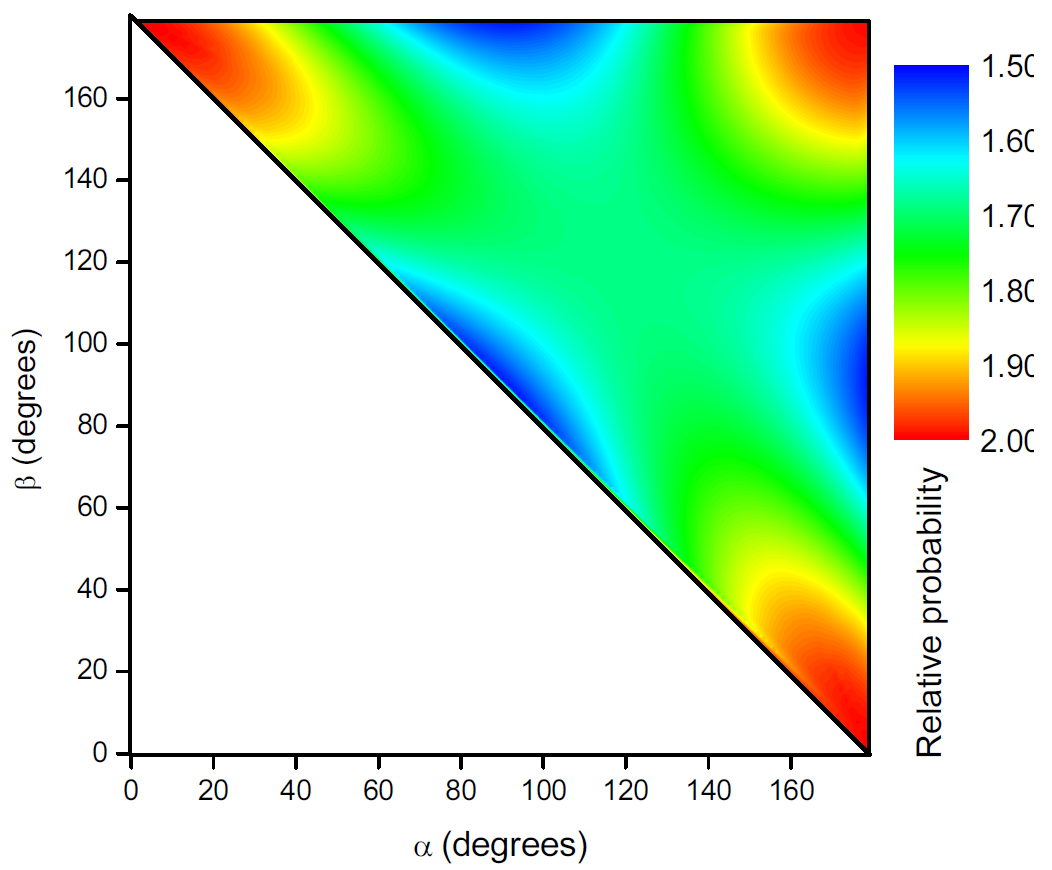
\includegraphics[width=15em]{immagini/3gamma_distribution}
	\caption{\label{fig:3gamma_angular_distr}Probabilità di una data distribuzione angolare per l'annichilazione a 3 fotoni. $\alpha$ e $\beta$ sono rispettivamente gli angoli tra il fotone 1 e i fotoni 2 e 3. La scala della probabilità e arbitraria.}
\end{figure}
%progettazione dell'esperimento

Una stima preliminare del rate di segnale atteso è ottenibile a partire dalla formula:
\begin{equation}
\label{eq:stima_3gamma}
R_{3\gamma} = R_{\beta^+} \cdot \frac{\text{BR}(3\gamma)}{\text{BR}(2\gamma)} \cdot 
\end{equation}


%realizzazione esperimento


%analisi